\documentclass[a0paper,portrait]{baposter}

\usepackage{xcolor}
\usepackage{wrapfig}
\usepackage{lmodern}
\usepackage{lipsum,graphicx}
\usepackage[utf8]{inputenc} %unicode support
\usepackage[T1]{fontenc}

\selectcolormodel{cmyk}

\graphicspath{{figures/}} % Directory in which figures are stored

\newcommand{\compresslist}{%
\setlength{\itemsep}{0pt}%
\setlength{\parskip}{1pt}%
\setlength{\parsep}{0pt}%
}

\newenvironment{boenumerate}
  {\begin{enumerate}\renewcommand\labelenumi{\textbf\theenumi.}}
  {\end{enumerate}}


\begin{document}

\definecolor{Mycolor1}{HTML}{B19D60} 

\definecolor{Mycolor2}{HTML}{FFDF00} 

\definecolor{Mycolor3}{HTML}{234DEB} 

\begin{poster}
{
grid=false,
headerborder=open, % Adds a border around the header of content boxes
colspacing=1em, % Column spacing
bgColorOne=white, % Background color for the gradient on the left side of the poster
bgColorTwo=white, % Background color for the gradient on the right side of the poster
borderColor=Mycolor1, % Border color
headerColorOne=Mycolor2, % Background color for the header in the content boxes (left side)
headerColorTwo=Mycolor2, % Background color for the header in the content boxes (right side)
headerFontColor=Mycolor3, % Text color for the header text in the content boxes
boxColorOne=white, % Background color of the content boxes
textborder=rounded, %rectangle, % Format of the border around content boxes, can be: none, bars, coils, triangles, rectangle, rounded, roundedsmall, roundedright or faded
eyecatcher=false, % Set to false for ignoring the left logo in the title and move the title left
headerheight=0.11\textheight, % Height of the header
headershape=rounded, % Specify the rounded corner in the content box headers, can be: rectangle, small-rounded, roundedright, roundedleft or rounded
headershade=plain,
headerfont=\Large\textsf, % Large, bold and sans serif font in the headers of content boxes
%textfont={\setlength{\parindent}{1.5em}}, % Uncomment for paragraph indentation
linewidth=2pt % Width of the border lines around content boxes
}
{}
%
%----------------------------------------------------------------------------------------
%	TITLE AND AUTHOR NAME
%----------------------------------------------------------------------------------------
%
{
  \textsf %Sans Serif
  {
    \hspace{-0.7cm}
    {CanAir.io}
  }
} % Poster title
% {\vspace{0.2em} Add Author Name, Add another author name\\ 
% {\small \vspace{0.7em} Department of Computing, TU Dublin, Tallaght, Dublin, Ireland}} 
{\sf\vspace{0.2em}\\
Antonio Vanegas  % Author names
\vspace{0.1em}\\
\small{ CanAirIO founder, Android-Hardware developer, Cos4Cloud member
\vspace{0.2em}\\
@hpsaturn  % Author email addresses
}
}
{
\includegraphics[width=.14\linewidth]{images/logo.png}} % CanAir.io logo


% this states the box starts at column 0 (edge of page), row 0 (top of page) for a span of 3 (columns wide)
\headerbox{CanAirIO Citizen Network for Air Quality Monitoring}{name=introduction,column=0,row=0, span=3}{
  This is an Open Source initiative that uses for now a ESP32 module and some kind
  PM2.5 sensors, interfaced with an Android client app to have static (WiFi) or mobile
  (Bluetooth) air quality stations. 
\vspace{0.5em}\\
  CanAirio is a citizen science iniciative that not only aims to generate an air
  quality network of fixed monitoring stations, but also to measure what occurs
  with pedestrians, drivers and passengers in their daily lives considering that
  in some cities the highest density of affected people is moving. For this
  reason, we are developing a mobile application that is able to set a PM2.5
  sensor, and other related sensors, as a fixed station using WiFi or mobile
  data from the smartphone by using a Bluetooth connection.

%\vspace{2cm} %remove this, only added for spacing

}

% this states the box starts at column 0 (edge of page), directly below the box labelled introduction for a span of 1 (column wide)
\headerbox{Main Goals}{name=subtopic1,column=0,below=introduction,span=1}{

%\vspace{0.15cm}

\vspace{5.0cm} %remove this, only added for spacing

}

% this states the box starts at column 0 (edge of page), directly below the box labelled subtopic1 for a span of 1 (column wide)

\headerbox{Countries}{name=subtopic2,column=0,below=subtopic1,span=1}{

  We want improve the DIY hardware and reduce the sensor complexity for that
  help a more people in the world.
  \vspace{0.1em}\\
  {
    \hspace{-0.1cm}
    \centering
    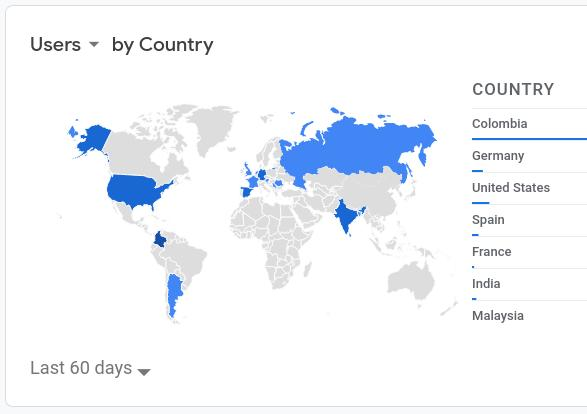
\includegraphics[scale=.28]{images/user_countries20200309.jpg}
  }
}

\headerbox{OpenSource and OpenHardware project}{name=subtopic3,column=1,below=introduction,span=2}{
\vspace{0.1cm}

% inserts an image inside the box, 5 rows high
\begin{wrapfigure}[4]{r}{0.5\textwidth}
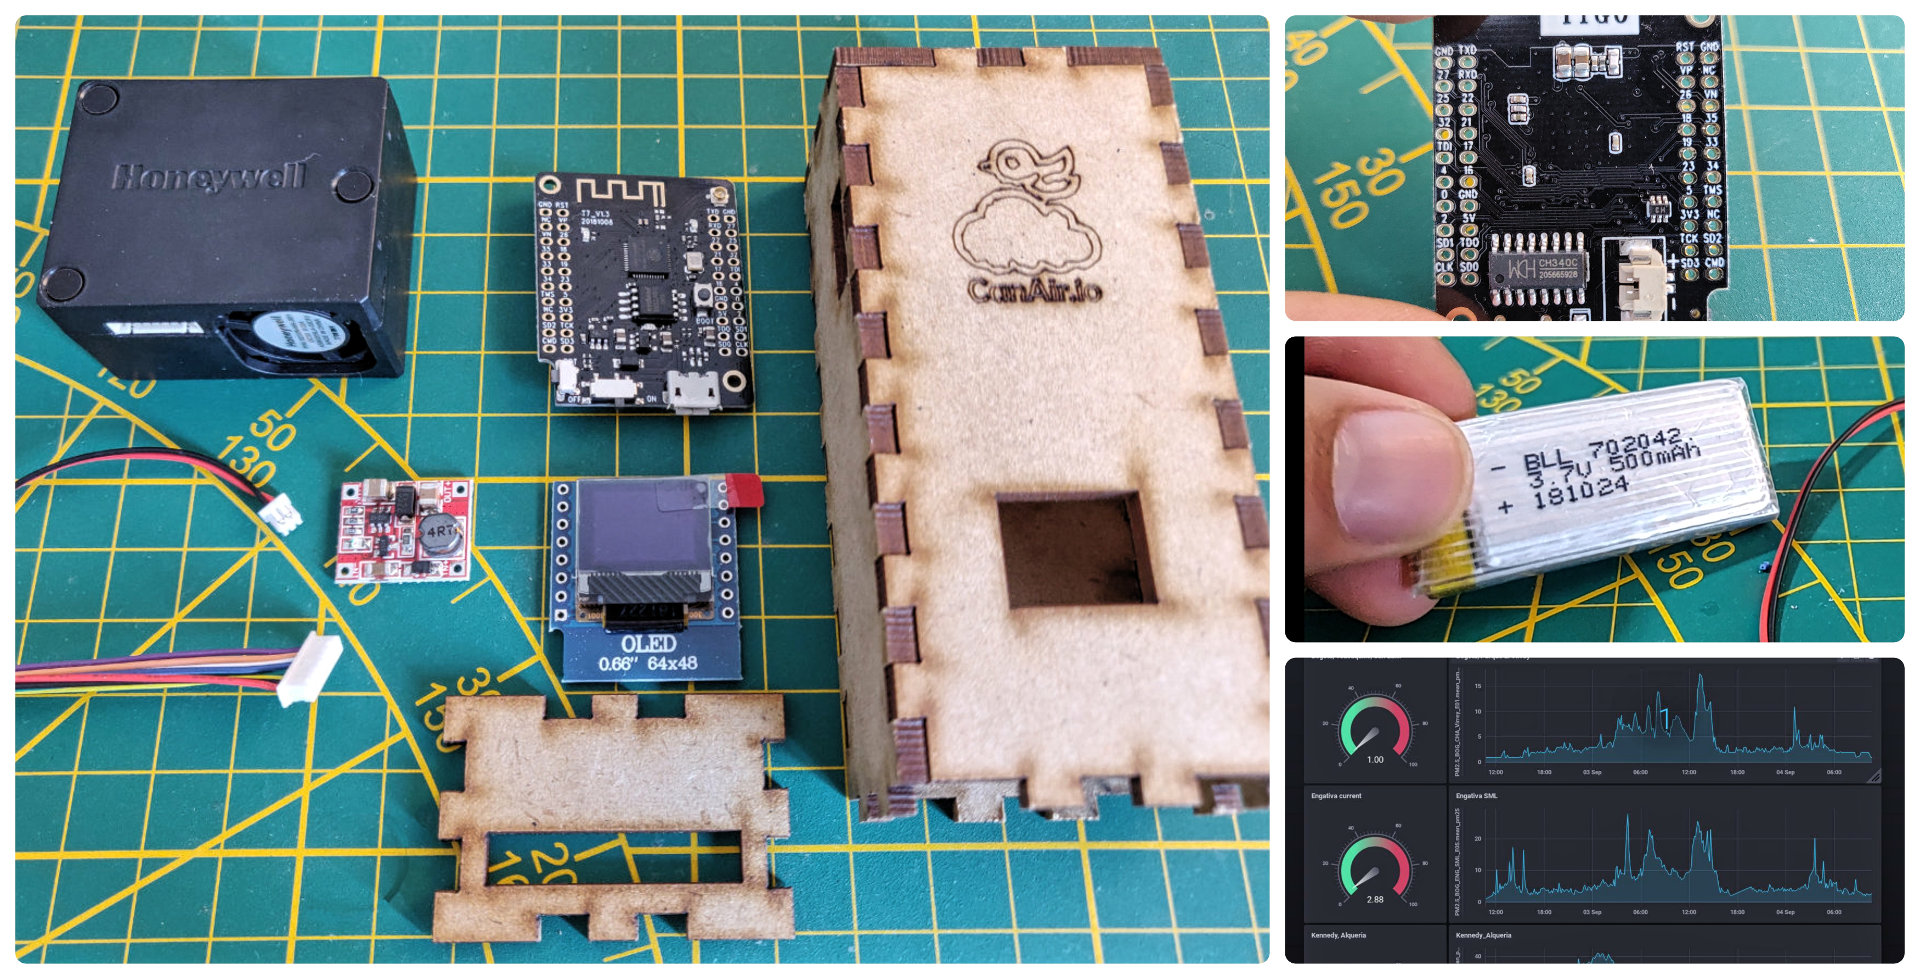
\includegraphics[width=1\linewidth]{images/canariov2collage01.jpg} 
\end{wrapfigure}

\subsubsection*{Hardware status:} 

- All firmware in PlatformIO framework.
\vspace{0.1em}\\
- GATT server for WiFi and Sensor setup.
\vspace{0.1em}\\
- Multiple sensor devices are supported.
\vspace{0.1em}\\
- Prototypes DIY with Laser cut boxes.
\vspace{0.1em}\\
- 3DPrint portatil case for mobile.

\subsubsection*{Software status:} 

- Android native application (GATT client)
\vspace{0.1em}\\
- InfluxDB cloud server for now.
\vspace{0.1em}\\
- API for writing, reading in development.
\vspace{0.1em}\\
- Web map for static stations.
\vspace{0.1em}\\
- Tool for show dinamic tracks for mobile captures. 
\vspace{0.1em}\\

% inserts an image inside the box, 5 rows high

{
  \hspace{0.1cm}
  \centering
  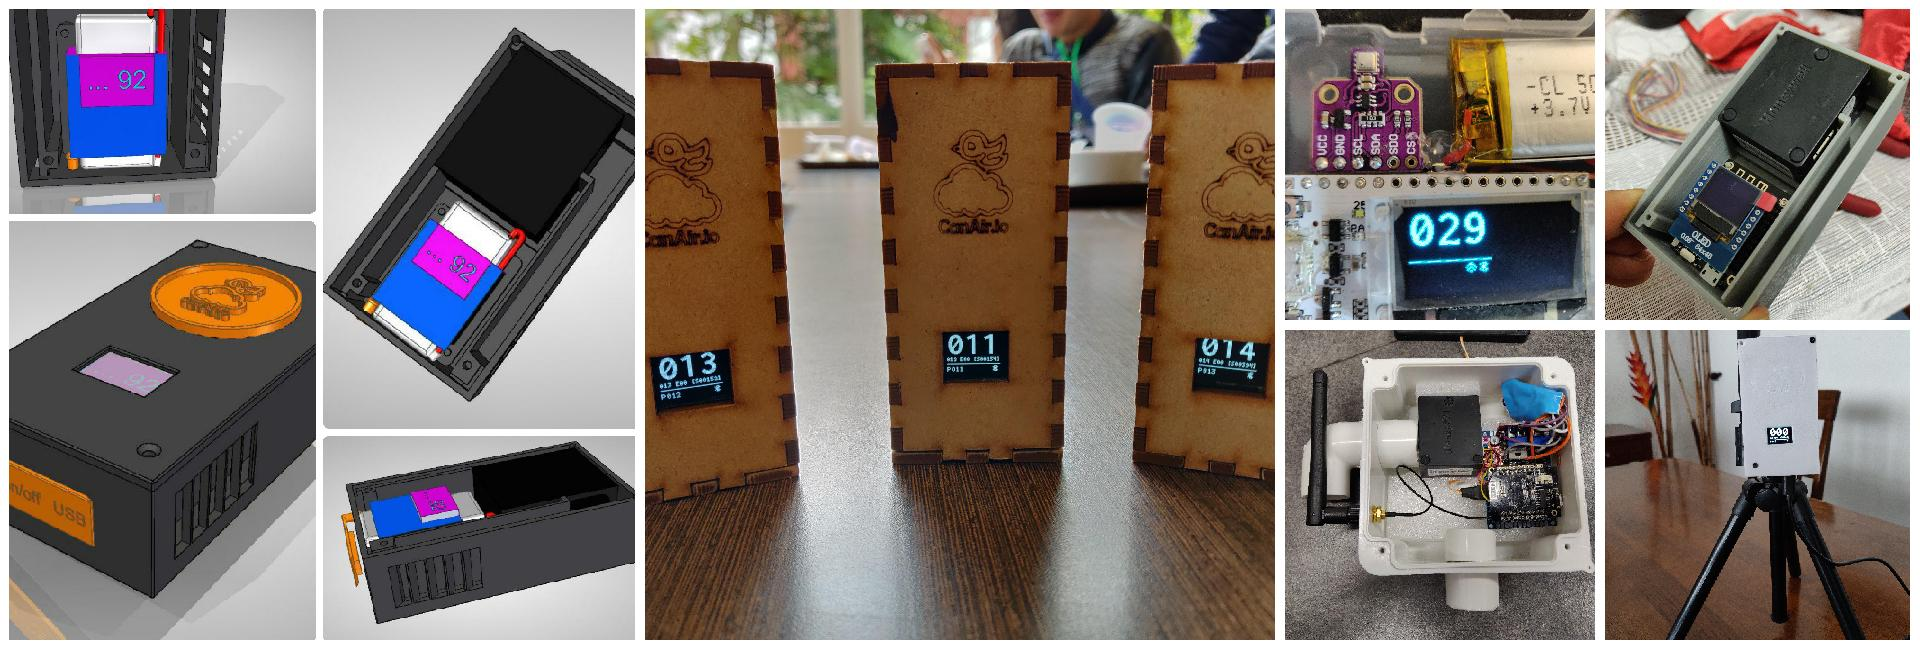
\includegraphics[width=.96\linewidth]{images/collage_horizontal02.jpg} 
}
\vspace{0.01cm} %remove this, only added for spacing
}


\headerbox{Citizen work and results}{name=topicoverview,column=0,span=3,below=subtopic2}{
{
    {
        \hspace{-.05cm}
        \centering
    	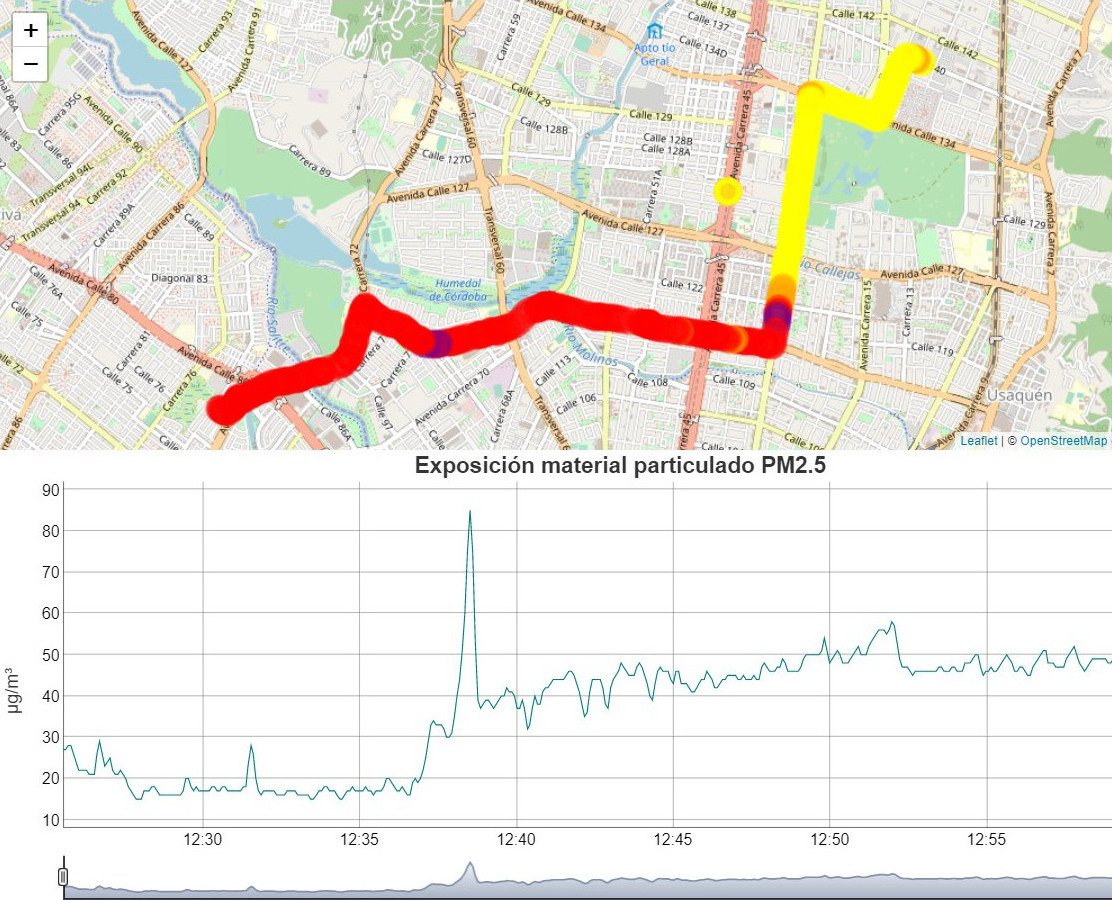
\includegraphics[scale=.82]{images/mobile_capture02.jpg}
    }
    {
        \hspace{-0.3cm}
        \centering
    	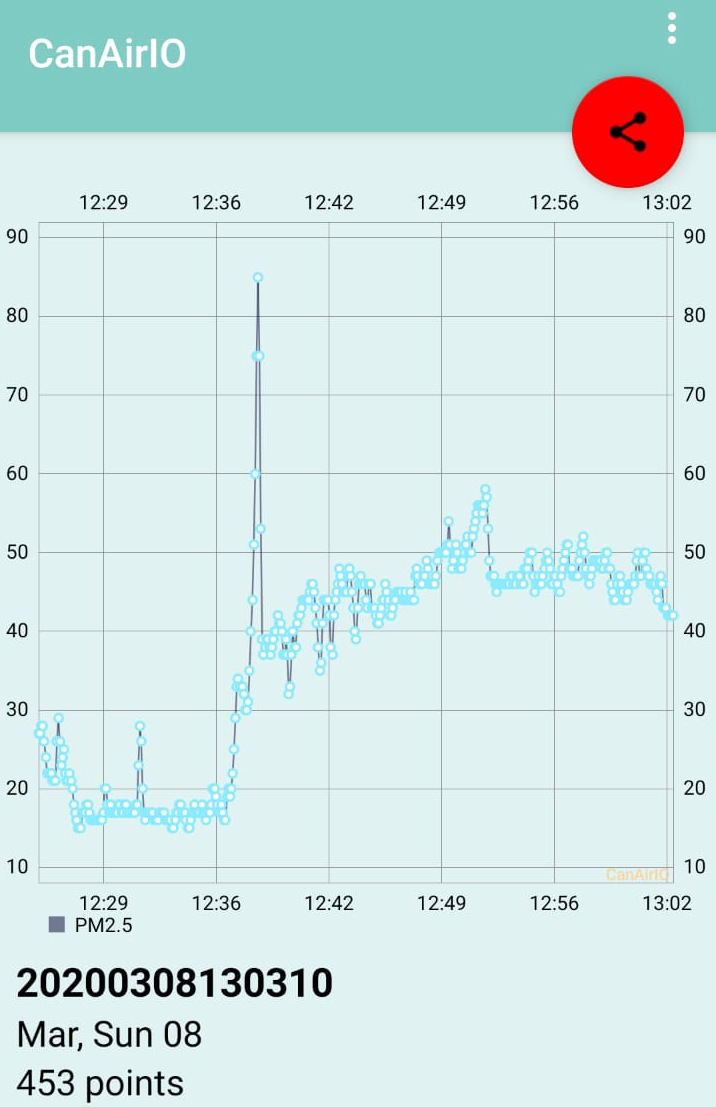
\includegraphics[scale=.15]{images/mobile_capture02_android.jpg}
    }
    {
        \hspace{-0.3cm}
        \centering
    	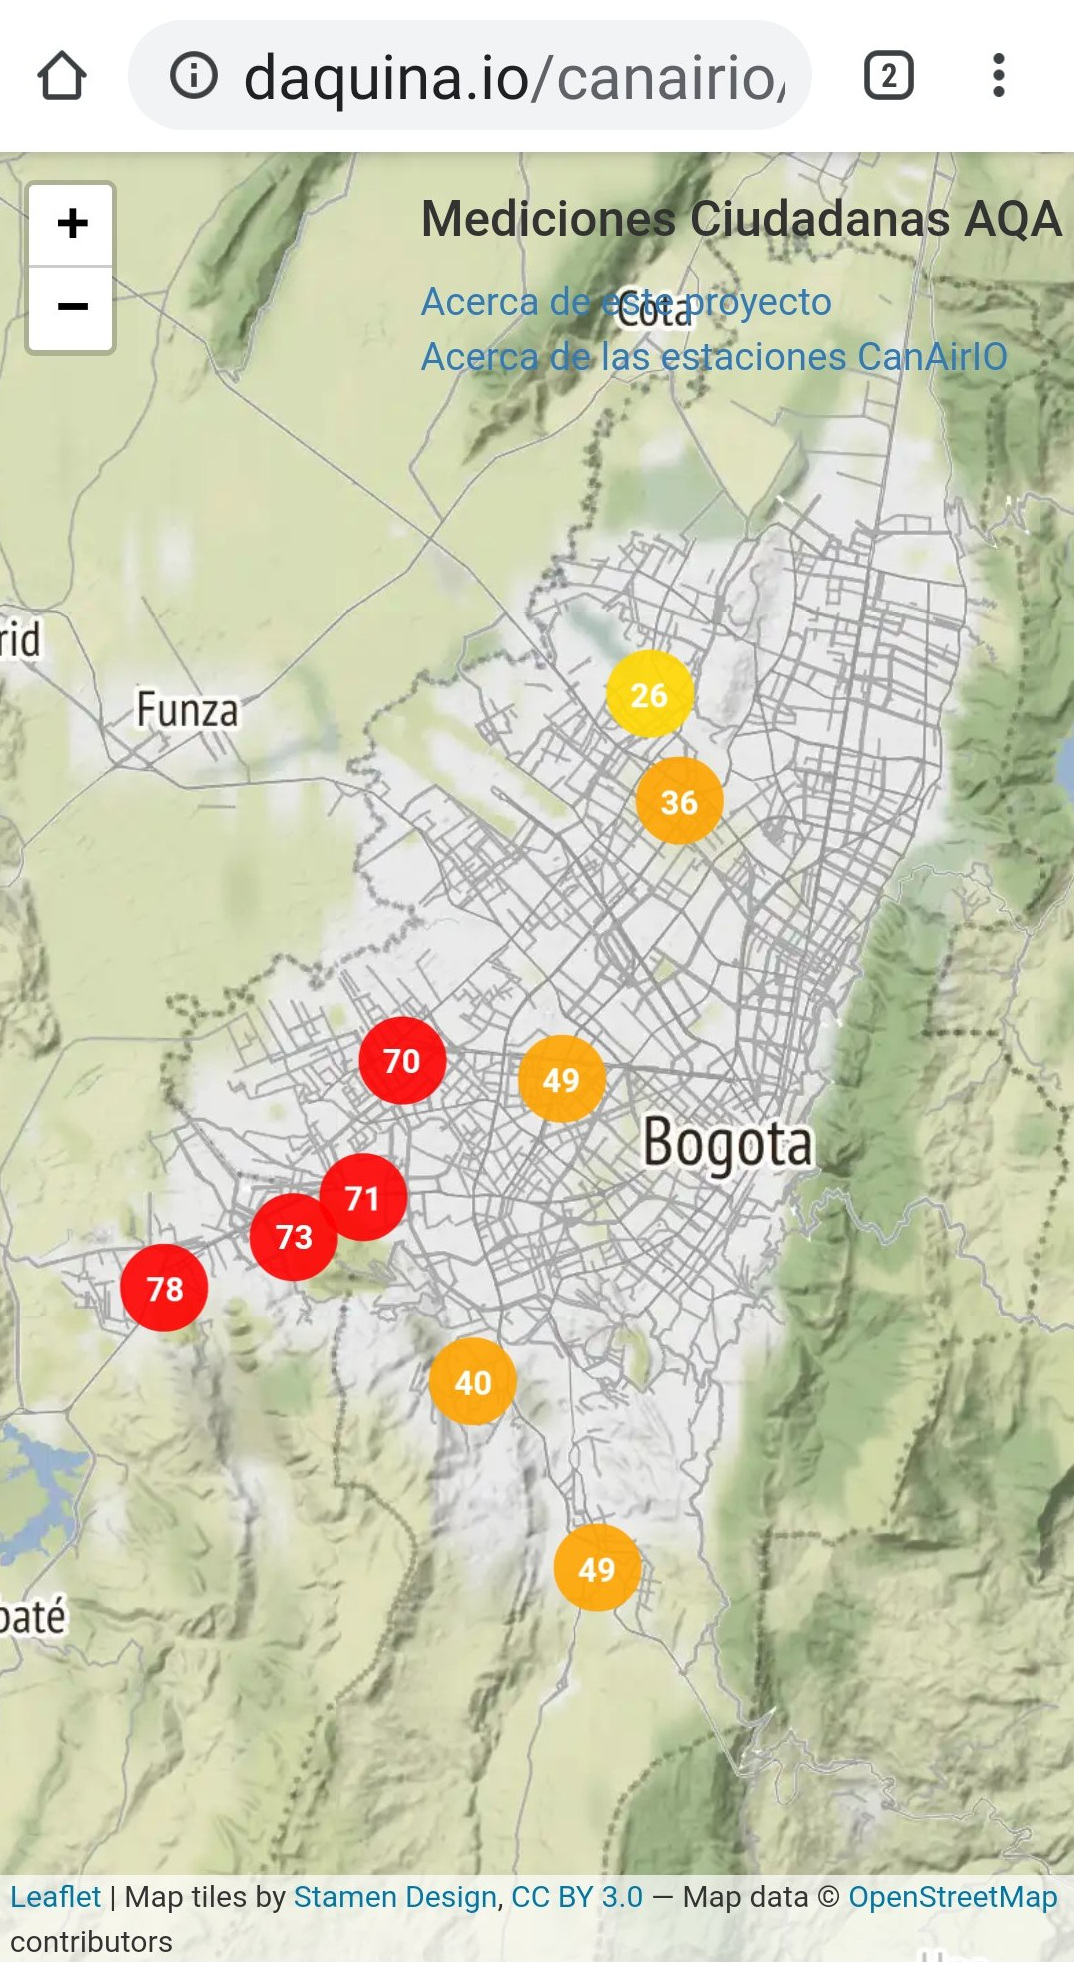
\includegraphics[scale=.078]{images/map_static_stations00.jpg}
    }
    {
        \hspace{-0.4cm}
        \centering
    	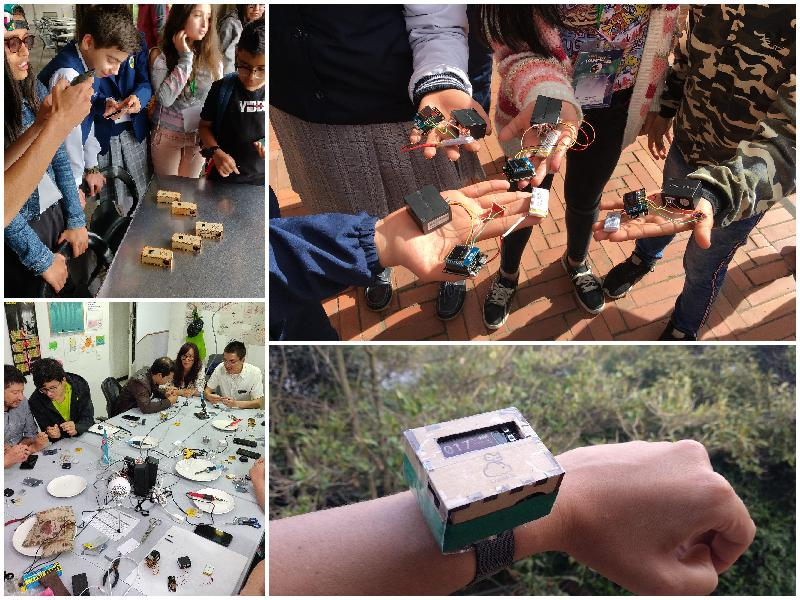
\includegraphics[scale=.3]{images/collage_square00.jpg}
    }
}

}

\headerbox{Thanks to:}{name=thanks,column=0,below=topicoverview,span=1,above=bottom}{

  {
    \subsubsection*{Sponsors:}
    Cos4Cloud: www.cos4cloud-eosc.eu
    \vspace{0.1em}\\
    Trébola: www.trebola.org
    \subsubsection*{Communities:}
    Hackbo: hackbo.co
    \vspace{0.1em}\\
    Unloquer: wiki.unloquer.org
    \vspace{0.1em}\\
    Grafoscopio: mutabit.com/grafoscopio
    \vspace{0.1em}\\
  }

}


\headerbox{Sponsors}{name=sponsors,column=1,below=topicoverview,span=2,above=bottom}{

  {
    {
        \hspace{0.2cm}
        \centering
      
\includegraphics[scale=.65]{images/trebola-logo-01.jpg}
    }
    {
        \hspace{-0.5cm}
        \centering
      
\includegraphics[scale=.14]{images/cos4Cloud_logo-02.png}
    }
    {
        \hspace{-0.5cm}
        \centering
      
\includegraphics[scale=.150]{images/https_canairio.png}
    }
  }

}
\end{poster}

\end{document}
